\title{LEZIONE 4 24/03/2020}\newline
\textbf{link} \href{https://web.microsoftstream.com/video/ddba4e0e-486c-4e25-9074-9749fa6a08f5?list=user&userId=8750338c-1a15-456b-9dc7-11c7358842b4}{clicca qui}
\subsection{Vincoli di contatto}
Proviamo ad analizzare il moto di un disco che rotola su una guida piana:\newline
[immagine dagli appunti del prof]
\begin{center}
    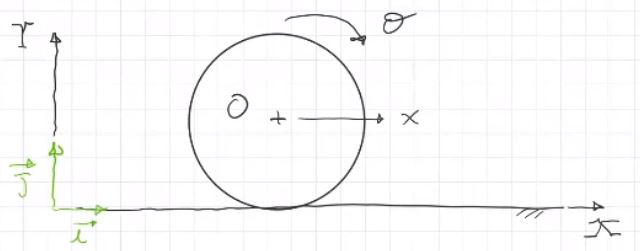
\includegraphics[height=3cm]{../lezione4/img1.JPG}
\end{center}
Notiamo subito che il centro $O$ del disco rigido si manterrà sempre a una distanza costante dalla guida piana, perciò $y_O = R = costante$: $v_{y_O} = 0$.\newline
\newline
Nell'analisi di sistemi con vincoli di contatto non è obbligatorio che che la velocità del punto di contatto si annulli: può essere presente una componente $v_{x_C} \neq 0$, che prende il nome di \textbf{velocità di strisciamento}.\newline
\newline
Da questo esempio notiamo che il vincolo di contatto introduce una sola equazione di vincolo che fa in modo che il disco abbia solo due gradi di libertà, $\theta$ e $x$.\newline
\newline
Il vincolo da imporre è quindi solo quello sul centro del disco:
\[
    \begin{cases}
        v_{y_O} = 0
    \end{cases}
\]
\subsection{Vincolo di puro rotolamento}
Nel caso di puro rotolamento non si ammette velocità di strisciamento, per cui i vincoli da imporre sono due:
\[
    \begin{cases}
        v_{y_O} = 0
    \end{cases}\;\;e\;\;\begin{cases}
        v_{y_C} = 0\\
        v_{x_C} = 0
    \end{cases}
\]
Notiamo che il punto di contatto $C$ rappresenta il punto di istantanea rotazione (CIR).
\newline
\newline
Nel vincolo di puro rotolamento abbiamo quindi due equazioni, di conseguenza si ha un solo grado di libertà, che può essere o $x$ o $\theta$.\newline
\newline
Vediamo ora il legame che c'è fra la coordinata $x$ e la coordinata $\theta$:\newline
[immagine dagli appunti del prof]
\begin{center}
    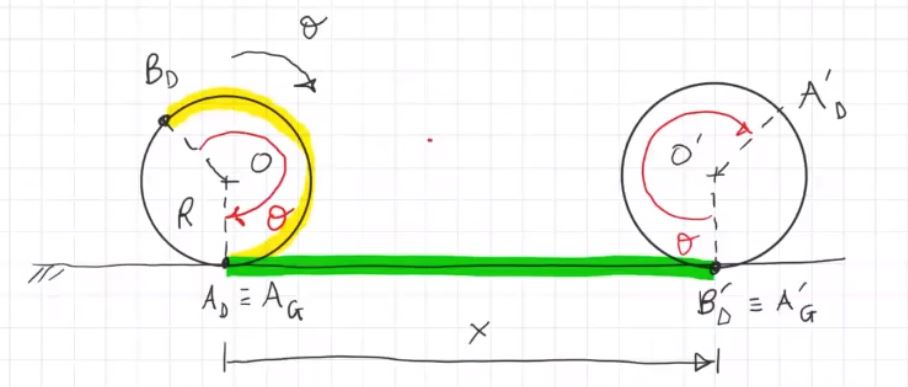
\includegraphics[height=4cm]{../lezione4/img2.JPG}
\end{center}
Notiamo subito che tutti i punti dell'arco $B_DA_D$ entreranno in contatto con la guida piana.\newline
Notiamo che il punto di contatto lungo la guida piana si sposta di una quantità $A_G A'_G$, che è la stessa quantità di $OO'$, e inoltre deve essere la stessa quantità dell'arco $B_D A_D$:
\[
    x = A_GA'_G = OO' = A_D B_D = \theta R
\]
\ \newline
Tenendo conto del risultato appena ottenuto e del vincolo sul centro del disco possiamo ottenere la legge oraria del centro del disco:
\[
    \begin{cases}
        x_O = \bar{X}_O + R \theta \;\text{(con $\bar{X}_O$ punto iniziale)}\;\\
        y_O = R
    \end{cases}
\]
Derivando possiamo trovare la velocità:
\[
    \begin{cases}
        v_{x_O} = R \dot{\theta} = \dot{x}\\
    v_{y_O} = 0
    \end{cases} \rightarrow \vec{v}_O = \vec{v} = R \dot{\theta} \vec{i}
\]
Derivando ancora troivamo l'accelerazione:
\[
    \begin{cases}
        a_{x_O} = R \ddot{\theta} = \ddot{x}\\
        a_{y_O} = o
    \end{cases} \rightarrow \vec{a}_O = R \ddot{\theta} \vec{i}
\]
La velocità angolare sarà invece calcolabile come $\vec{\omega} = \omega \vec{k} = \dot{\theta} \vec{k}$, che sarà negativa perchè il disco ruota in senso orario (regola della mano destra). Sfruttando Rivals possiamo ricavare la velocità di un generico punto $P$ interno al disco:\newline
[immagine dagli appunti del prof]
\begin{center}
    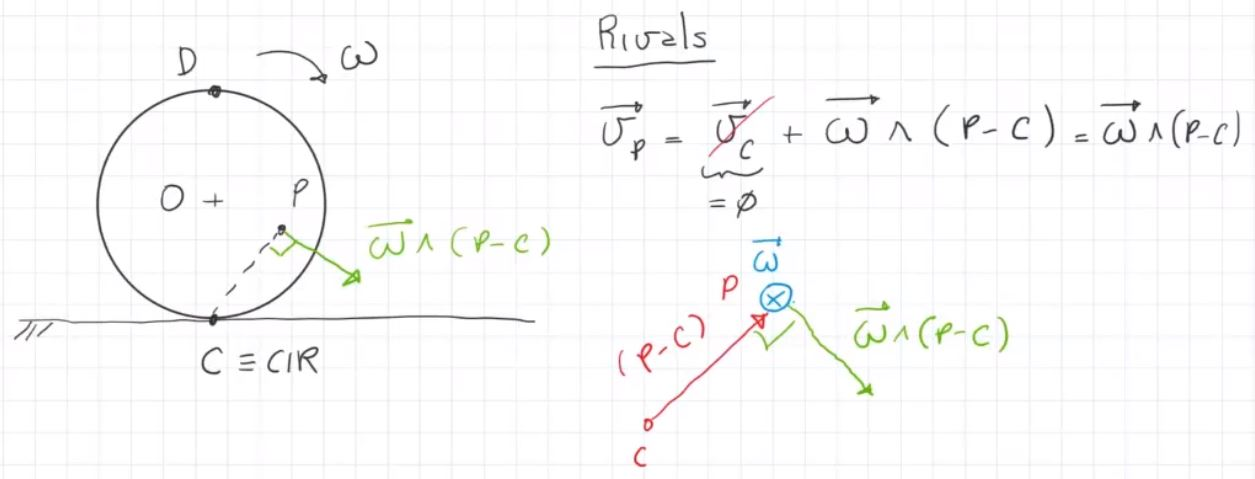
\includegraphics[height=4cm]{../lezione4/img3.JPG}
\end{center}
Allo stesso modo (con Rivals) possiamo calcolare la velocità del centro del disco o del punto diametralmente opposto al punto di contatto:\newline
[immagine dagli appunti del prof]
\begin{center}
    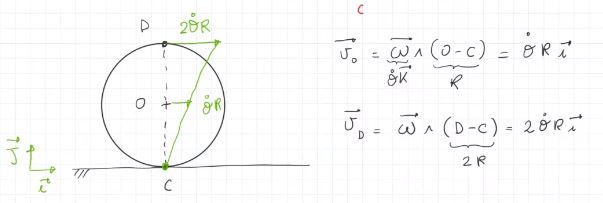
\includegraphics[height=4cm]{../lezione4/img4.JPG}
\end{center}
Sappiamo che il punto di contatto è il centro di istantanea rotazione, quindi ha velocità nulla, ma accelazione diversa da zero, andiamo a calcolare l'accellarazione. Sapendo che l'accellerazione del centro $\vec{a}_O = \ddot{\theta} R \vec{i}$, grazie a Rivals otteniamo che
\[
    \vec{a}_C = \vec{a}_O + \dot{\vec{\omega}} \land (C-O) + \vec{\omega} \land[\vec{\omega} \land (C-O)] = \vec{\omega} \land[\vec{\omega} \land (C-O)]
\]
siccome $\vec{a}_O = \ddot{\theta} R \vec{i}$ e $\dot{\vec{\omega}} \land (C-O) = - \ddot{\theta} R \vec{i}$, rimane quindi la sola accellerazione normale che è uguale a:
\[
    \vec{a}_C = \dot{\theta}^2 R \vec{j}
\]
[immagine dagli appunti del prof]
\begin{center}
    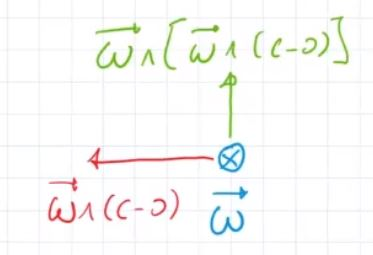
\includegraphics[height=3cm]{../lezione4/img5.JPG}
\end{center}
\ \newline
Da notare che tutti i calcoli fatti si potevano ritrovare analizzando il sistema con un sistema di coordinate in modo relativo posto sul centro del disco.
\newpage
\section{Cinematica dei sistemi meccanici}
\subsection{Classificazione dei sistemi meccanici}
I sistemi meccanici possono essere classificati in due macro categorie:
\begin{itemize}
    \item \textbf{Meccanismi}: Si definisce meccanismo un sistema meccanico in cui vi è almeno una possibilità di moto residua una volta imposti vincoli. In poche parole il numero di gradi di libertà deve essere maggiore o uguale a $1$.
    \item \textbf{Struttura}: Il sistema non ha nessun grado di libertà, le uniche possibilità di movimento sono legate alle deformabilità dei corpi.
\end{itemize}
All'interno di questo corso vedremo solo meccanismi.\newline
\newline
I mecanismi a loro volta si suddividono in due sottocategorie:
\begin{itemize}
    \item \textbf{Catene cinemaitca aperte}: Ciascun corpo che costituisce il sistema è collegato esclusivamente al corpo che lo precede o al corpo che lo segue dalla catena (telaio incluso).
    \item \textbf{Catene cinemetiche chiuse}: Se non è aperta.
\end{itemize}
La differenza fra questi due sistemi è che nel caso di catene aperte, per studiare il moto di un corpo è sufficiente studiare il moto relativo di un corpo rispetto a quello che lo precede, viceversa in una catena chiusa il moto del meccanismo si userà un'\textbf{equazione} detta \textbf{di chiusura}.\newline
\newline
L'\textbf{equazione di chiusura} esprime utilizzando il formalismo dei numeri complessi il poligono chiuso che in ogni istante del moto è descritto dalla catena cinematica chiusa.
\subsubsection{Regola di Grublen}
La \textbf{Regola di Grublen} si usa per calcolare quanti gradi di libertà abbia un sistema meccanico \textbf{piano} con \textbf{vincoli elementari} che ciascuno colleghi \textbf{al più due corpi} (eccezione fatta per i telai).\newline
\newline
Il numero $n$ di gradi di libertà è dato dalla regola:
\[
    n = 3 \cdot n_c - n_v = 3 \cdot n_c - (1 \cdot n_1 + 2 \cdot n_2 + 3 \cdot n_3)
\]
con $n_c$ il numero di corpi rigidi; $n_v$ il numero di vincoli, $n_1$ il numero di vincoli singoli, $n_2$ il numero di vincoli doppi e $n_3$ il numero di vincoli tripli.\newline
\newline
Ovviamente bisogna sempre tenere conto che il numero di gradi di libertà è sempre maggiore o uguale a $0$.\newline
\newline
Se utilizzando la regola di Grublen il numero di gradi di libertà è esattamente $0$, allora siamo in presenza di una struttura \textbf{isostatica}, se il numero di gradi di libertà risulta essere negativo, allora siamo in presenza di una struttura \textbf{iperstatica}.
\newpage
\section{Cinematica del manipolatore SCARA}
\subsection{Introduzione}
[immagini dagli appunti del prof]
\begin{center}
    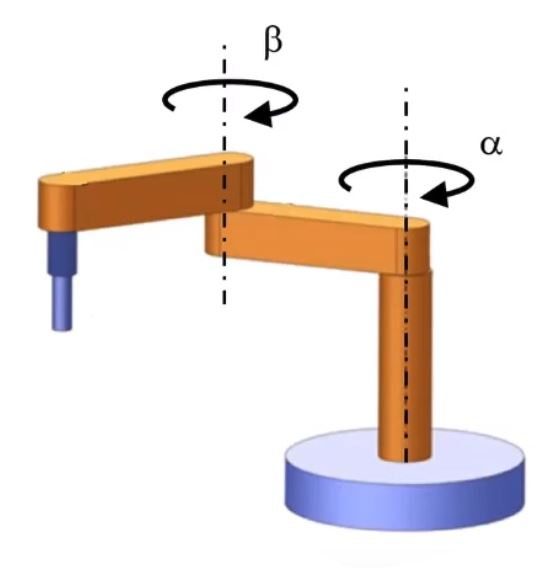
\includegraphics[height=3cm]{../lezione4/img7.JPG}
\end{center}
\begin{center}
    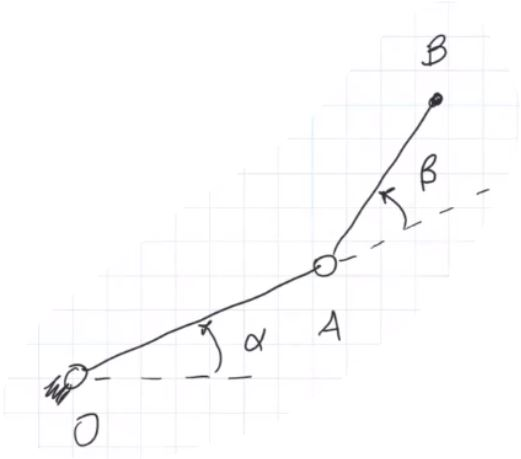
\includegraphics[height=3cm]{../lezione4/img8.JPG}
\end{center}
Il manipolatore \textbf{SCARA} ha due gradi di libertà che sono $\alpha$ e $\beta$ ed è una \textbf{catena cinematica aperta}. Il punto $B$ prende il nome di \textbf{end-effector} ed è il punto di interesse. Per studiarlo bisogna conoscere in ogni istante l'evoluzione di $\alpha(t)$ e $\beta(t)$ nel tempo e le loro derivate.\newline
\newline
\subsection{Numeri complessi}
Analiziamo il sistema SCARA col formalismo dei numeri complessi:\newline
[immagine dagli appunti del prof]
\begin{center}
    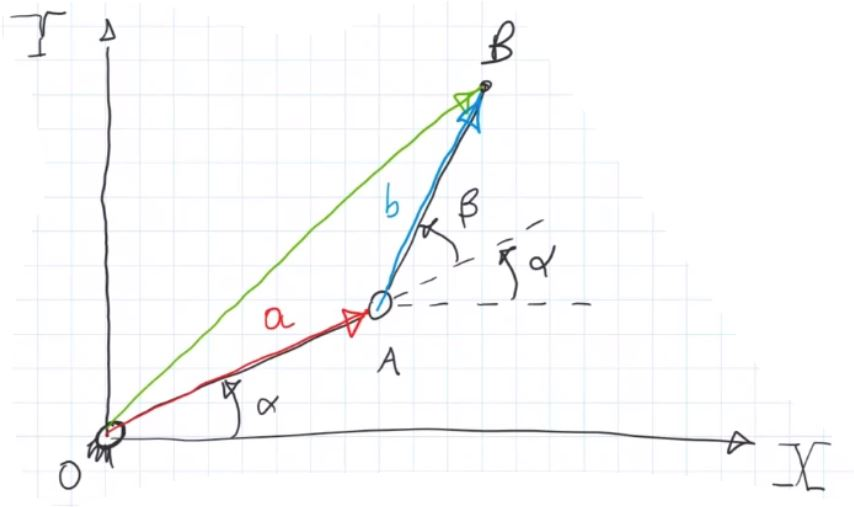
\includegraphics[height=4cm]{../lezione4/img9.JPG}
\end{center}
Per studiare la \textbf{posizione} del punto $B$ possiamo sommare le posizioni delle due aste $OA$ e $AB$:
\[
    (B-O) = (A-O) + (B-A) = a e^{i \alpha} + b e^{i(\alpha + \beta)}
\]
Passiamo ora in forma parametrica:
\[
    \begin{cases}
        x_B = a cos(\alpha) + b cos(\alpha + \beta)\\
        y_B = a sin(\alpha) + b sin(\alpha + \beta)
    \end{cases}
\]
Derivando otteniamo la \textbf{velocità}:
\[
    \vec{v}_B = \frac{d}{dt} (A-O) + \frac{d}{dt} (B-A) = i a \dot{\alpha} e^{i \alpha} + i b (\dot{\beta} + \dot{\alpha}) e^{i(\alpha+\beta)} = a \dot{\alpha} e^{i(\alpha + \frac{\pi}{2})} + b (\dot{\beta} + \dot{\alpha})e^{i(\alpha + \beta + \frac{\pi}{2})}
\]
\[
    \begin{cases}
        \dot{x}_B = -a \dot{\alpha} sin(\alpha) - b (\dot{\alpha} + \dot{\beta})sin(\alpha + \beta)\\
        \dot{y}_B = a \dot{\alpha} cos(\alpha) + b (\dot{\alpha} + \dot{\beta}) cos(\alpha + \beta)
    \end{cases}
\]
[immagine dagli appunti del prof]
\begin{center}
    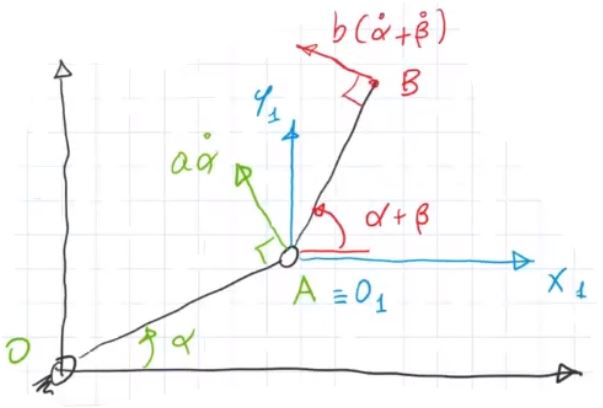
\includegraphics[height=3cm]{../lezione4/img10.JPG}
\end{center}
Deriviamo ancora per l'\textbf{accellerazione}:
\[
    \vec{a}_B = a \ddot{\alpha} e^{i(\alpha + \frac{\pi}{2})} - a \dot{\alpha}^2 e^{i \alpha} + b (\ddot{\alpha} + \ddot{\beta})e^{i(\alpha + \beta + \frac{\pi}{2})} - b (\dot{\alpha} + \dot{\beta})^2 e^{i(\alpha + \beta)}
\]
da cui possiamo ricavare la forma parametrica facendo le proiezioni (...).\newline
\newline
Andiamo ad analizzare i termini che compongono l'accellerazione:
\begin{itemize}
    \item $\vec{a}_{tr,B} = a \ddot{\alpha} e^{i(\alpha + \frac{\pi}{2})} - a \dot{\alpha}^2 e^{i \alpha}$ sono rispettivamente la componente tangenziale e quella normale dell'accellerazione di trascinamento di $B$. (In verde nell'immagine).
    \item $\vec{a}_{rel,B} = b (\ddot{\alpha} + \ddot{\beta})e^{i(\alpha + \beta + \frac{\pi}{2})} - b (\dot{\alpha} + \dot{\beta})^2 e^{i(\alpha + \beta)}$ sono rispettivamente la componente tangenziale e la componente normale dell'accellerazione relatica rispetto al sistema di riferimento con centro in $A$. (In rosso nell'immaigne).
    \item Notiamo che dal teorema dei moti relativi ($\vec{a} = \vec{a}_{tr} + \vec{a}_{rel} + \vec{a}_{co}$), manca il termine dell'accellerazione di Coriolis, che però siccome abbiamo scelto una terna traslante la velocità angolare della terna è nulla e quindi il termine di Coriolis si annulla.
\end{itemize}
[immagine dagli appunti del prof]
\begin{center}
    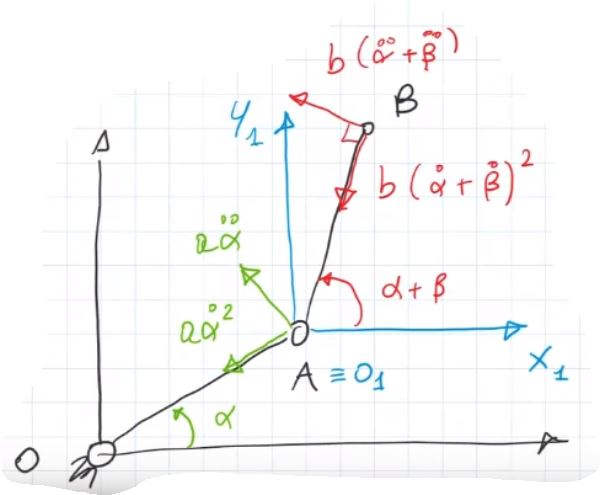
\includegraphics[height=4cm]{../lezione4/img11.JPG}
\end{center}
Interpretiamo ora i risultati ottenuti col teorema dei moti relativi, in particolare consideriamo le seguenti due possibili configurazioni: traslante e rotante. [impostiamo il problema, lasciamo la soluzione come compito dello studente].
\subsection{Sistema mobile traslante}
Poniamo un sistema mobile traslante con origine nel punto $A$ e traslante sulla sua traiettoria circolare.\newline
\newline
[immagine dagli appunti del prof]
\begin{center}
    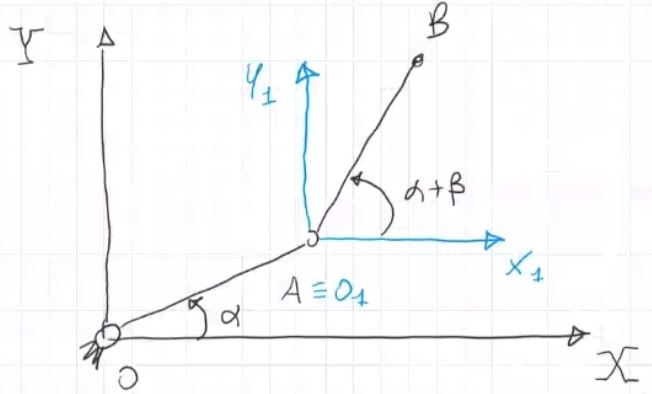
\includegraphics[height=3cm]{../lezione4/img12.JPG}
\end{center}
Accellerazione angolare della terna: $\omega_t = \dot{\omega}_t = 0$.\newline
Accellerazione di Coriolis: $\vec{a}_{co} = 2 \vec{\omega}_t \land \vec{v}_{rel,B} = 0$.\newline
\newline
Utiliziamo ora i teoremi dei moti relativi per calcolare velocità e accellerazioni:\newline
$\vec{v}_B = \vec{v}_{tr,B} + \vec{v}_{rel,B}$ e $\vec{a}_B = \vec{a}_{tr,B} + \vec{a}_{rel,B} + \vec{a}_{co}$.\newline
\newline
Notiamo che la velocità angolare dell'asta $AO$ è pari a $\vec{\omega}_{AO} = \dot{\alpha} \vec{k}$ (con $\alpha$ angolo fra l'asse delle $X$ e l'asta $AO$), mentre la velocità angolare dell'asta $BA$ è pari a $\vec{\omega}_{BA} = (\dot{\alpha} + \dot{\beta}) \vec{k}$ (con $\alpha + \beta$ angolo fra l'asse $X_1$ e l'asta $AB$).\newline
\newline
[terminare a casa, soluzione nel pdf della lezione]
\subsection{Sistema mobile rotante}
Poniamo un sistema mobile rotante con origine nel punto $A$ e rotante solidalmente all'asta $OA$.\newline
\newline
[immagine dagli appunti del prof]
\begin{center}
    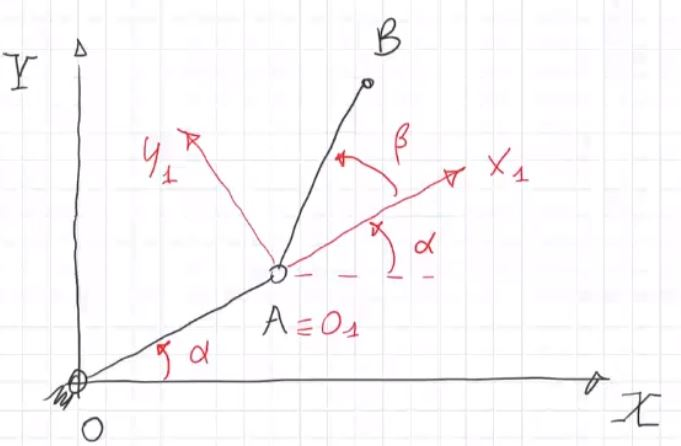
\includegraphics[height=3cm]{../lezione4/img13.JPG}
\end{center}
Accellerazione angolare della terna: $\vec{\omega}_t = \dot{\alpha} \vec{k}$, $\dot{\vec{\omega}} = \ddot{\alpha} \vec{k}$.\newline
Accellerazione di Coriolis: $\vec{a}_{co} \neq 0$.\newline
\newline
Notiamo che la velocità angolare dell'asta $AO$ è pari a $\vec{\omega}_{AO} = \dot{\alpha} \vec{k}$ (come il caso precedente), mentre la velocità angolare dell'asta $BA$ è pari a $\vec{\omega}_{BA} = \dot{\beta} \vec{k}$.\newline
\newline
La velocità relativa di $B$ diventa $\vec{v}_{rel,B} = \vec{\omega}-{BA} \land (B-A) = \dot{\beta} e^{i(\alpha + \beta + \frac{\pi}{2})}$.\newline
\newline
[terminare a casa, soluzione nel pdf della lezione]